\chapter{Literature Review}\label{C:review}

In this chapter, we first introduce the background of web service composition in Section \ref{overview}.  Followed that Section \ref{} discuss the single-objective service composition for both EC and non-EC based approaches. Section  \ref{} reviews existing works in muti-objective approaches and many-objective approaches.  Dynamic web service composition is covered in Section \ref{}. Section \ref{}  discussed most AI planning-based approaches to semantic service composition. Lastly, Section \ref{} summarises some critical points discussed in this chapter as well as some inadequacies or limitations in the literature review.
\section{Background}\label{background}

\subsection{Web Service}\label{service}
Web services are self-describing modules offering functionalities over the internet. The functionalities of web services are often specified by their functional attributes, which satisfy users' functional requirements and provide mechanisms to allow users to search desired service. Web services are classified into two groups based on their functionalities:  \emph{information-providing services} and \emph{world-altering services} \cite{mcilraith2001semantic}. The first type of services expect some data returned by giving inputs or nothing. For example, a service for air velocity transducer reads the wind speed and return the velocity at the time. This service does not require any inputs. On the other side, a service for city weather requires given city name to return the weather information for that specific city. Information-providing services do not produce any side effect to the world. The functionalities of these services are only inputs and outputs. The second type of services not only provide data information but also alters the status of the world by producing side effects. For example, a PayPal service will cause a deduction in the balance of users' bank account. \emph{In this proposal, we mainly focus the first type of services for first three objective. Later on, an extensive study is optimally carried on the second type of services}

In realistic scenarios, the non-functional are also important. For example, users may not prefer a service with higher cost with the same functionality provided by another one. As demonstrated above, the functional attributes determine what service really does, while the non-functional attributes often refers to some quality criteria, which is considered for raking services \cite{agarwal2009making}. We first explain web services using a formal model from \cite{agarwal2010d5} below, where both the functional and non-functional attributes are captured uniformly. Further, A Labelled Transition System \cite{agarwal2009making} is addressed with its abstract and updated model for demonstrating the behaviours of web services in Subsection \ref{functional}, which emphasises on side of the functional attributes. After demonstrating these models, we will discuss about the nonfunctional properties of web services in Subsection \ref{nonfunctional}.

\textbf{A Formal Model of Web Service}. Given a finite set $\wp$ of property types of web services and a finite set $\vartheta$ of values sets. Each property type is associated with a value set. We view a Web service as a finite set $Q$ of property instances with each property instance $q \in Q$ being of a property type$t(q) \in \wp$ that is associated with a value $v_q \in \vartheta_{t(q)}$. See Fig. \ref{fig:ws}

\begin{figure}
\centerline{
\fbox{
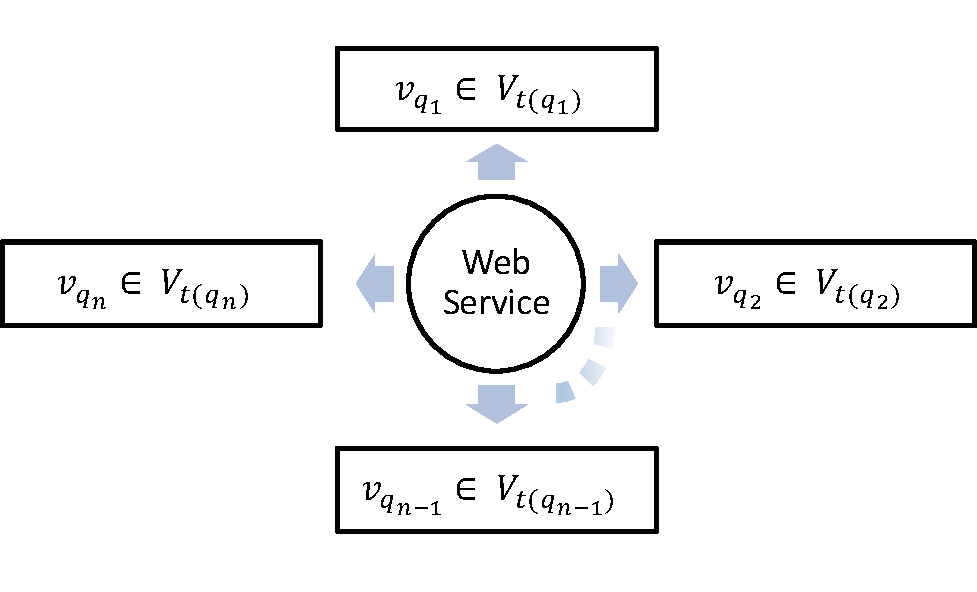
\includegraphics[width=8cm]{ws.pdf}
}}
\caption{Property-Based Web Service Formal Model \cite{agarwal2010d5}.}
\label{fig:ws}
\end{figure}

\subsubsection{Functional Properties of Web services}\label{functional}

\textbf{A Functionality Model}. This mode is represented as a Labelled Transition System (LTS): $L = (S,T,\rightarrow)$ comprises a set $S$ of states, a set $T$ of transition labels and a labeled transition relation $\rightarrow \subseteq S \times T \times S$. This transition system is established to present the actual behaviour of web services, which consists of a series of states. See Fig. \ref{fig:lts}.

\begin{figure}
\centerline{
\fbox{
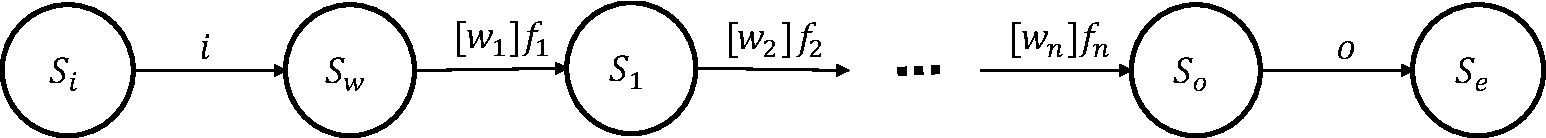
\includegraphics[width=14cm]{LTS.pdf}
}}
\caption{ The functionality of a Web Service \cite{agarwal2010d5}.}
\label{fig:lts}
\end{figure}

\begin{itemize}
\item $S_i$ start state includes knowledge available to web service before the web service is invoked by inputs; 
\item $S_w$ state includes the inputs additional to the knowledge in 1; 
\item A series of state $S_1$ to $S_n$ proceed with corresponding actions $f_n$ that only occurred if each related condition $[w_i]$ is approved to be true. 
\item $S_o$ state contains all the outputs and all the changes performed in the knowledge base. 
\item $S_e$ is the end state, which is equivalent to $S_o$, since the knowledge base is not changed.
\end{itemize}

\textbf{An Abstract Functionality Model}. The first functionality model presented above is not completely demonstrated for the internal actions, as the services provider does not want reveal all the internal functions, and it is not feasible to list a global set of property name. Therefore, an abstract functionality of a web service is modelled by eliminating all the intermediate properties. In the abstract model of a web service, the functional properties of the web service could be identified as inputs $i$, pre-state $S_i$, outputs $o$ and post-state $S_o$. These four properties are mapped to a set of input $I$, preconditions $\phi$, a set of outputs $O$ and postcondition $\varphi$ respectively in third updated functionality model demonstrated below.

\textbf{A Updated functionality Model}. In the updated model, a set of inputs $I$ is required by a service and a set of output $O$ is returned after the successful execution. Apart from that, the precondition $\phi$ must be hold in the knowledge base before service is invoked by passing the input $I$. To enable the interoperability of the functional properties, ontology reasoner is employed to reason about the properties of web services. To distinguish the changes between before and after service execution, these changes are modelled as property instances. For example, inputs and outputs assigned as variable names and further referenced in preconditions and postconditions, which can be distinguished as different instances from the knowledge base. In particular, preconditions is assigned to the description of requirements of inputs using logic formula. Herein the description of the formula considers the following cases that are demonstrated using Planning Domain Description Language (PDDL \cite{fox2003pddl2}):
\begin{itemize}
\item Conditions on the type of inputs, e.g., the payment of an online shopping website is made by Visa or Cash: $\phi:(Format(payment)=Visa \cup Format(payment)=Cash)$.
\item Relationships among inputs, e.g.,  authoried users are required for an online shopping: $\phi:(Authoried ? Useraccount)$.
\item Conditions on the value of inputs, e.g., saving account balance has more than 100 dollars: $\phi: (\geq (amounts, saving account), 100)$
\end{itemize}
These preconditions must be hold in the state consistently while inputs are being passed to services. Similarly, the postcondition is restricted to the description of constraints on returned outputs, relationships between inputs and outputs, and changes caused by the service in the knowledge bases.

\subsubsection{Nonfunctional Properties of Web services}\label{nonfunctional}
Apart from the functional properties of web services discussed above, the non-functional properties of web services play an important part in composing services. For example, customers prefer lowest execution cost with highest response time and reliability. According to \cite{zeng2003quality}, four most often considered QoS parameters are as follows:
\begin{itemize}
\item \textit{Response time} ($T$) measures the expected delay in seconds between the moment when a request is sent and the moment when the results are received.
\item \textit{Cost} ($C$) is the amount of money that a service requester has to pay for executing the web service
\item \textit{Reliability} ($R$) is the probability that a request is correctly responded within the maximum expected time frame.
\item \textit{Availability} ($A$) is the probability that a web service is accessible.
\end{itemize}

\subsubsection{Web Service Discovery}\label{servicediscovery}
To generate service compositions, web service must provide mechanisms for discovery required services. Therefore, service discovery must be one fundamental technique to be considered in all service composition approaches. \cite{agarwal2009d5} discussed three mechanisms of semantic web service discovery: classification-based approach, functionality-based approach and hybrid approach. Those service discovery techniques are further demonstrated below.

The first service discovery technique makes use of the classes provided by service semantic annotation in WSMO-Lite language. Therefore, service requesters can use class names to express a goal offering a straightforward discovery from a set of classes. However, classes without clear meaning definition could lead to the issue of incomprehensibility of web service discovery. For example, several classes may declared in either different terms for the describing the same content or same terms for describing different content.

The second service discovery technique  does not take classes into account, but consider functional properties of web service to include pre-conditions and post-conditions. In particular, a desired functionality description is defined. A discovery algorithm must be developed to handle a matching for different input, output, precondition and postcondition with associated concepts and relations in the provided domain knowledge base. The key idea of the matchmaking is to check whether services accept all the desired inputs provided bu users and whether the desired outputs is delivered by services. In addition, the matchmaking algorithm also checks for the satisfiability of implications that actual precondition and actual postcondition must imply the desired precondition and desired postcondition respectively. The strength of the second is that it potentially meet the demands of all the comprehensible discovery, while the weakness is a lack of efficiency and scalability. 

The third service discovery technique is based on a hybridisation of classification and functionality-based discovery. Classification hierarchy is proposed to achieve automatic semantic reasoning in hierarchical functionality. For example, a functionality class is associated with super classes and sub classes for more general functionality class and more specific functionality class respectively. However, to make a consistency of classification hierarchy, the inputs, outputs, precondition and postcondition of a functionality class must satisfy the conditions that contains all the inputs, outputs, precondition and postcondition of all the classes it is subsumed by. The advantage of this approach is to achieve better performance combining strengths of the previous two pure classifications based and functionality based approaches. While the classification hierarchy needs to be kept consistent when a new web service is published or updated.​

As discussed above, the first and third approach is considered either less effective or demands to build up a consistent ontology for classes and their functional attributes. That is not the focus of our research.  \emph{In the proposal, we use the second service discovery technique for meeting the comprehensible discovery. That is, different types of ontology reasoning are utilised to approach the matchmaking as a fundamental part of service composition algorithm.}



\subsection{Web Service Composition}\label{overview}

Since one atomic web service could not satisfy or fully satisfy users' complex requirements, web service composition is approached by composing web services together with more sophisticated functionalities to meet the demand. Due to fully human intervention in manual service composition, so it is very time-consuming and less productive. Therefore, many approaches have been developed to achieve semi-automated or fully automated service composition. The semi-automated service composition is inspired by the business process that required prior knowledge to build up the abstract workflow. This workflow can be decomposed into several functional services slots for proper services being fitted. These steps are further discussed in Subsection \ref{lifecycle}. On the other hand, when we are composing services, both semi-automated and fully automated web service composition holds the challenge in the interoperability of services discussed previously. In particular, several problems are simultaneously taken into account. That is I/O matchmaking (i.e., the mechanisms of services for ensuring the interoperability ), discovery relevant services to the optimising the quality of service composition, e.g., overall QoS. Consequently, the following concerns are required to consider in generating composition solution. 


\subsubsection{Web Service Composition Lifecycle}\label{lifecycle}
Typical steps in a workflow-based automated Web service composition solution are shown in Fig. \ref{fig:lifecycle}. The detail of the service lifecycle is discussed as follows:

\begin{figure}
\centerline{
\fbox{
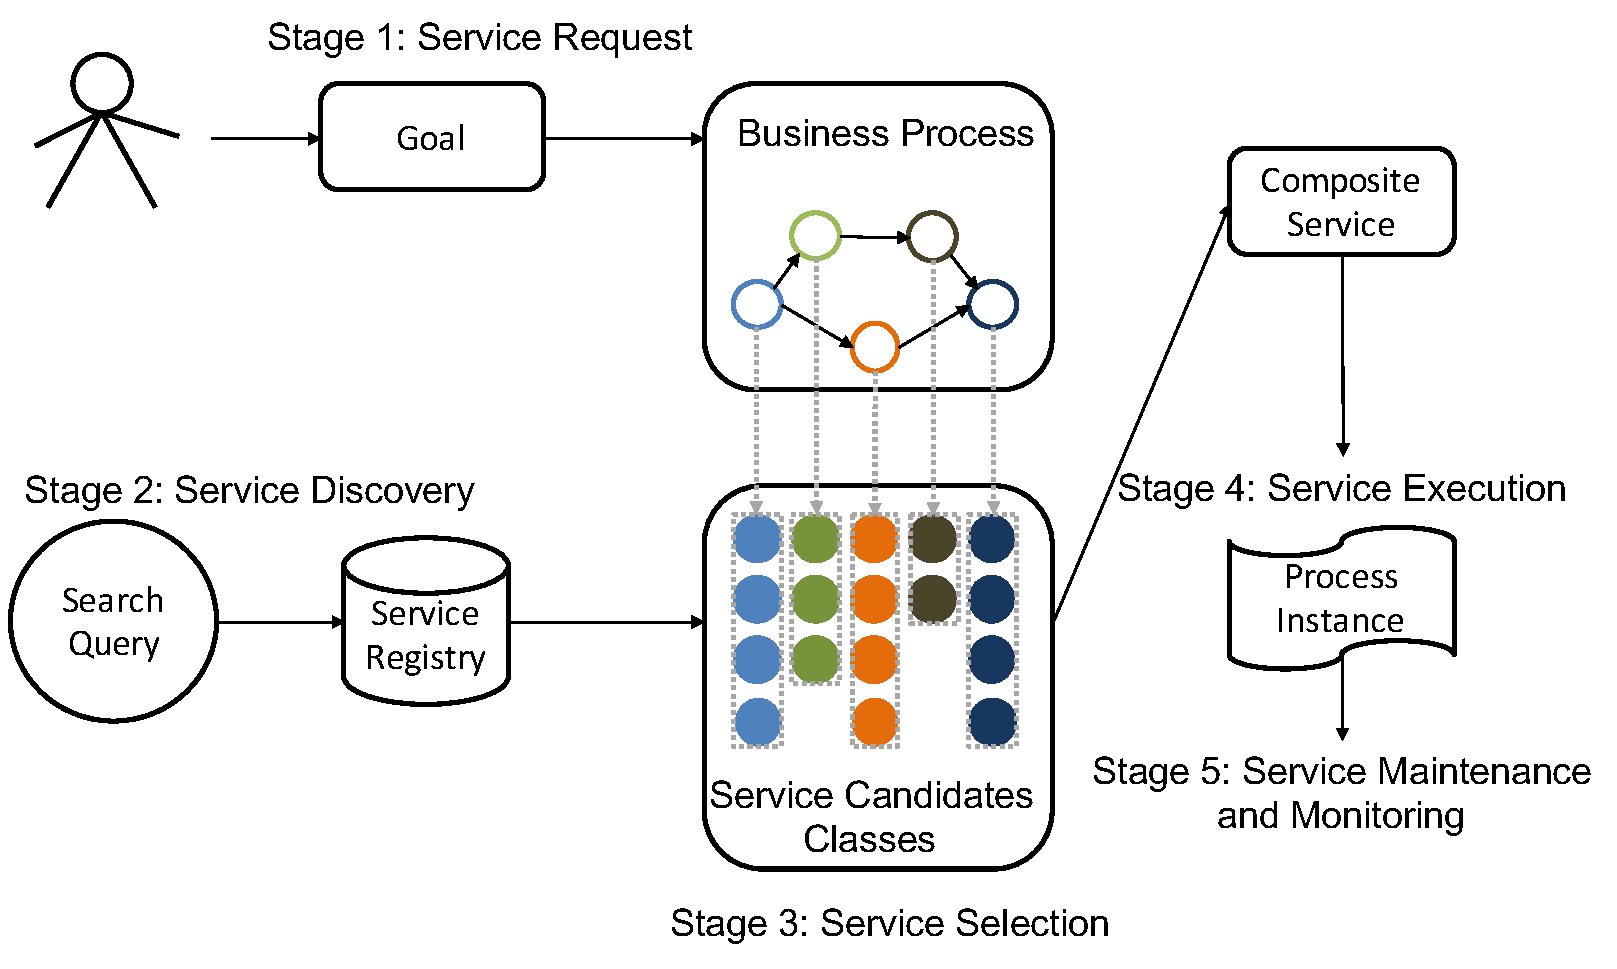
\includegraphics[width=14cm]{compositionLifecycle.pdf}
}}
\caption{ Web service composition lifecycle \cite{moghaddam2014service}.}
\label{fig:lifecycle}
\end{figure}

\begin{enumerate}
 \item \textit{Goal specification:} The first step in service composition is to collect users' requirements for composition goal that comprises of the functional (i.e., correct data flow ) and non-functional side (i.e., QoS). This step is achieved by building up an abstract workflow including a series of tasks with clearly defined functionality. Those tasks could be completed by selecting proper concrete services to reach desired QoS. 
 \item \textit{Service discovery:} Once the goal is clearly specified, concrete web services are to be selected for each task regarding its functional requirement. Often, more than one concrete web service is likely to be found to match the one task. However,  those matched web services are always different in QoS.  Therefore, web services are classified by the functionality of each task, i.e., inputs and outputs.
 \item \textit{Service selection:} At this stage, many techniques have been studied to select web services to best match each task for the satisfying functional requirement of each task and overall business process. Therefore, a plan of service composition is created ahead of execution.

 \item \textit{Service execution:} the process instance is monitored for any changes or services failures during service execution. In this stage, some actions are to be taken for adapting the changes.
\end{enumerate}
The web service lifecycle discussed above is a typical \emph{semi-automated approach}. There is a distinction between semi-automated and fully automated approaches. On the one hand, during the goal specification stage of semi-automated approach, the abstract work is already provided.  On the other hand, an abstract workflow is not provided at the stage of goal specification for \emph{fully automated service composition}. Often, fully automated service composition rely on some algorithms (e.g., Graphplan algorithm \cite{blum1997fast}) to achieve service composition, during which service workflow is gradually built up along with the service discovery and service selection at the same time. In this proposal, I concentrate on developing methods for fully automated service composition since it has been shown the flexibility. Also, herein service discovery and service selection are considered as interrelated tasks that are interleaved with the composition algorithm.

\subsubsection{Functional Properties of Web Service Composition}
Substantial work \cite{bansal2016generalized,lecue2009optimizing, lecue2007making, lecue2006formal, rao2005semantic} on semantic web service composition utilises Description logic (DL) reasoning between input and output parameters of web services for matchmaking. OWL and OWL-S are the most common semantic specifications used currently \cite{petrie2016web}, and they enable automatic selection, composition, and interoperation of Web services to implement complicated composition tasks \cite{martin2004owl}. However, some matchmaking types (discussed below) may penalise the matchmaking quality and are less preferred by users. Therefore, exploring a effective mechanism for measuring the quality of semantic matchmaking in service composition is a very demanding research area.

Given two concepts $a, b$ in ontology $\mathcal{O}$, four commonly used \emph{Matchmaking types} are often used to describe the level of a match between outputs and inputs \cite{paolucci2002semantic}: 
\begin{itemize}
\item the \emph{matchmaking} returns $exact$ if $a$ and $b$ are equivalent ($a \equiv b$), 
\item the \emph{matchmaking} returns $plugin$ if $a$ is a sub-concept of $b$ ($a \sqsubseteq b$),
\item the \emph{matchmaking} returns $subsume$ if $a$ is a super-concept of $b$ ($a \sqsupseteq b$), 
\item the \emph{matchmaking} returns $fail$ if none of previous matchmaking types is returned. 
\end{itemize}

Often, the similarity of two instances of two knowledge representations encoded in the same ontology is also utilised to measure the quality of matchmaking regarding the four matchmaking types discussed above. The work \cite{lecue2007making} additionally consider $interaction$ matchmaking type ($a \sqcap b$), i.e., if the intersection of $a$ and $b$ is satisfiable. In their work, a causal link link \begin{math} sl_{i,j} \stackrel{.}{=} \langle S_i, Sim_{T}(Out\_s_i,In\_s_j),S_j  \rangle \end{math} is created between two functional property instances for a input and a output. In particular, both $exact$ match and $plugin$ match are presented as robust causal links, while both $subsume$ match and $intersection$ match are presented as valid casual links. However, valid casual links are not specific enough to be utilised as the input of another web service. Thus the output requires Extra Description Equation \ref{equation2} to enable proper service composition. As a result, Subsume and Intersection matching type is transferred to be Exact and PlugIn respectively to formulate a robust link. 

\begin{equation}
In\_s_x \setminus Out\_s_y \stackrel{.}{=} \underset {\preceq d}{min} \{ B|B\sqcap  Out\_s_y \equiv In\_s_x  \} , since \  Out\_s_y \sqsupseteq In\_s_x
 \label{equation2}
\end{equation}



\emph{In this paper we are only interested in robust compositions where only $exact$ and $plugin$ matches are considered, see \cite{lecue2009optimizing}. As argued in \cite{lecue2009optimizing} $plugin$ matches are less preferable than $exact$ matches due to the overheads associated with data processing. We suggest to consider the semantic similarity of concepts when comparing different $plugin$ matches.} Herein we demonstrate an example of a robust causal link by between two matched services $S$ and $S'$, noted as $S \rightarrow S'$, if an output $a$ ($a \in {O_S}$) of $S$ serves as the input $b$ ($b \in {O_{S'}}$) of $S'$ satisfying either $a \equiv b$ or $a \sqsubseteq b$.  For concepts $a, b$ in $\mathcal{O}$ the \emph{semantic similarity} $sim(a, b)$ is calculated based on the edge counting method in a taxonomy like WorldNet or Ontology \cite{shet2012new}. This method has the advantages of simple calculation and good performance \cite{shet2012new}. Therefore, the \emph{matchmaking type} and \emph{semantic similarity} of a robust causal link can be defined as follow:

\begin{align}
\label{eq_link}
type_{link} = 
\begin{cases}
	1 & \text{ if $a\equiv b$ ($exact$ match)}\\
	p & \text{ if $a \sqsubseteq b$ ($plugin$ match)}
\end{cases}
,&&
sim_{link} = sim(a,b) = \frac{2N_c}{N_{a}+N_{b}}
\end{align}

\noindent with a suitable parameter $p, 0<p< 1$, and with $N_a$, $N_b$ and $N_c$, which measure the distances from concept $a$, concept $b$, and the closest common ancestor $c$ of $a$ and $b$ to the top concept of the ontology $\mathcal{O}$, respectively. However, if more than one pair of matched output and input exist from service $S$ to service $S'$, $type_e$ and $sim_e$ will take on their average values.

The \emph{semantic matchmaking quality} of the service composition can be obtained by aggregating over all robust causal links as follow:
\begin{align}
MT {=} \prod_{j=1}^{m} type_ {link_{j}}
,&&
SIM {=} \frac{1}{m}\sum_{j=1}^m sim_ {link_{j}}  
\end{align}


\subsubsection{Nonfunctional Properties of Web Service Composition}
The nonfunctional properties of web service composition is determined by all the QoS of involved concrete web services in the solution. The aggregation value of QoS attributes for web services composition varies with respect to different constructs, which reflects how services associated with each other in a service composition \cite{zeng2003quality}.

We use formal expressions as in \cite{ma2012formal} to represent service compositions. We use the constructors $\bullet$, $\parallel$, $+$ and $\ast$ to denote sequential composition, parallel composition, choice, and iteration, respectively. The set of \emph{composite service expressions} is the smallest collection $\mathcal{SC}$ that contains all atomic services and that is closed under sequential composition, parallel composition, choice, and iteration. That is, whenever $\cse_0,\cse_1,\ldots,\cse_d$ are in $\mathcal{SC}$ then $\bullet(\cse_1,\ldots,\cse_d)$, $\parallel(\cse_1,\ldots,\cse_d)$, $+(\cse_1,\ldots,\cse_d)$, and $\ast \cse_0$ are in $\mathcal{SC}$, too. Let $\cse$ be a composite service expression. If $\cse$ denotes an atomic service $S$ then its QoS is given by $QoS_S$.  Otherwise the QoS for $\cse$ can be obtained inductively as summarized in Table~\ref{tbl:QoS_Aggre}. Herein, $p_1,\ldots,p_d$ with $\sum\limits^d_{k=1}p_k=1$ denote the probabilities of the different options of the choice $+$, while $\ell$ denotes the average number of iterations.

\begin{table}[htb]
\centering
\caption{QoS calculation for a composite service expression $\cse$}
\begin{tabular}{l|l|l|l|l}
\hline
 $\cse=$       &$r_\cse=$                              &$a_\cse=$                              &$c_\cse=$                            &$t_\cse=$ \\ \hline
 $\bullet(\cse_1,\ldots,\cse_d)$      &$\prod\limits^d_{k=1}r_{\cse_k}$    &$\prod\limits^d_{k=1}a_{\cse_k}$    &$\sum\limits^d_{k=1}c_{\cse_k}$   &$\sum\limits^d_{k=1}t_{\cse_k}$  \\ \hline
 $\parallel(\cse_1,\ldots,\cse_d)$  &$\prod\limits^d_{k=1}r_{\cse_k}$    &$\prod\limits^d_{k=1}a_{\cse_k}$    &$\sum\limits^d_{k=1}c_{\cse_k}$   &$MAX \{ t_{\cse_k} | k \in \{ 1,...,d \} \}$\\ \hline
 $+(\cse_1,\ldots,\cse_d)$     &$\prod\limits^d_{k=1}p_k\cdot r_{\cse_k}$    &$\prod\limits^d_{k=1}p_k\cdot a_{\cse_k}$    &$\sum\limits^d_{k=1}p_k\cdot c_{\cse_k}$   &$\sum\limits^d_{k=1}p_k\cdot t_{\cse_k}$  \\ \hline
 $\ast \cse_0$         &${r_{\cse_0}}^\ell$  &${a_{\cse_0}}^\ell$  &$\ell\cdot c_{\cse_0}$ &$\ell\cdot t_{\cse_0}$ \\ \hline
\end{tabular}
\label{tbl:QoS_Aggre}
\end{table}

\subsection{Evolutionary Computation Techniques Overview}\label{problem}

Evolution Computing (EC) techniques are founded based on the principles of Darwin natural selection. The nature evolution and selection of individual in a population are automated simulated in EC. In particular, a population of individuals is initialised for directly or indirectly presenting the solutions. Those individual candidates are evolved and evaluated using a fitness function to evaluate the degree of how good (or bad) of each individual. Therefore, it is possible to reach solution with near-optimal fitness. EC have been shown its promise in solving combinatorial optimisation problems \cite{back1997evolutionary}. This is due to its flexibility in encoding the problems for the representation and its good performance in many scenarios. In particular, To manage the constrainsts in the problems, five main methods have been proposed deal with the constraints: coding, penalty functions, repair algorithm, indirect methods of representation and multiobjective optimisation \cite{fleming2002evolutionary}. In the context of service composition. Many EC techniques have been approached for handling optimisation problems for web service composition, such as Genetic Algorithms (GA) \cite{whitley1994genetic}, Genetic Programming (GP) \cite{koza1992genetic}, Particle Swarm Optimisation (PSO) \cite{kennedy1995particle}, and Clonal Section Algorithm \cite{de2002learning}. These techniques are briefly introduced here.

GP is considered as a particular application of GA with a set of different encoded genes. In particular, the representation of GA is commonly represented as a linear structure. However, In GP, each individual is commonly represented as a tree structure. the tree structure has a terminal set and a function set, where variables, constants and functions are consisted of respectively. Also,  the tree structure is considered be efficiently evaluated recursively. Three genetic operators consisting of reproduction, crossover, and mutation are involved in to generate next generation for both GA and GP. Reproduction operator retains the elite individual without any changes. Crossover operator replaces one node of one individual with another node of another individual. Mutation operator replaces a randomly selected node in an individual. The whole evaluation process won't stop unless an optimised solution found or a pre-defined number of generation reached.

PSO is one of swarm intelligence (SI) that based on the behaviour of decentralized, self organised system. PSO algorithm is initialised by a group of random particles, which direct or indirect present the solutions. Those particles explores for the optimisation position, which is approached by repeating the process of transferring particles position according to both their own best-known position and global best position.

Artificial immune system (AIS) has been studied for performing machine learning, pattern recognition and solving optimisation problems.  Clonal Section Algorithm (CSA) is one of AIS for handling optimisation problems, and the principle of utilising Clonal Section Algorithm lie in the features of immune memory, affinity maturation. In particular, the antigen is considered as a fitness function instead of the explicit antigen population, and a proportion of antibody, rather than the best affinity antibody, are chosen to proliferation. Further more, speed and accuracy of the immune response grow higher and higher after each infection even confronting cross-reactive response. Apart from that, hypermutation and receptor editing contribute to avoiding local optimisation and selecting optimised solution respectively. 


\section{Related Work}\label{related}

\subsection{Single-Objective Web Service Composition Approaches}\label{SingleObjective}

In this section, approaches to QoS-aware web service composition is to be discussed in two distinct groups: EC-based approaches, which mainly rely on the EC techniques to reach the optimal solutions, and Non-EC based methods, which do not utilise any bio-inspired methods. However, most of these approaches employ a single-objective fitness function for optimising a united QoS score as a simple Additive Weighting (SAW) technique \cite{hwang1981lecture}.
\subsubsection{EC-based Composition Approaches}
EC-based web service composition mainly relies on evolutionary computation algorithms for searching optimal solutions. These algorithms are inspired by the behaviour of human, animals or even T-cells.  To cope with different EC algorithms, proper representations are to be designed for direct or indirect represent the service composition solutions. Herein we mainly discuss some promising research works on QoS-aware web service composition using  Genetic Algorithm (GA), Genetic Programming (GP), Particle Swarm Optimisal (PSO), and Clonal Selection Algorithm (CSA).

\textbf{Genetic Algorithm}. 
GA is a very reliable and powerful technique for solving combinatorial optimisation problems \cite{srinivas1994genetic}. It has been applied to handle optimisation problems for QoS-aware web service composition \cite{wang2012survey}. \cite{canfora2005approach} developed a GA-based approach for semi-automated QoS-aware service composition, where an abstract workflow is given. In their work, GA methods are compared to linear integer programming. The experimental finding reveals GA method is preferred when the size of service candidates are increasing.  \cite{tang2010hybrid} proposed a hybrid approach utilising GA and local search. In particular, a local optimizer is developed and only recalled in the initial population for improving QoS value. This local search contributes to a better overall performance compared with GA-methods without local search. In \cite{lecue2009optimizing},  a semi-automated service composition approach is developed in their paper for optimising the quality of semantic matchmaking and some quality criteria of QoS. In particular, the quality of matchmaking problem is transferred to measure the quality of semantic links, which is proposed by two quality aspects: matchmaking type and degree of similarity.

\textbf{Genetic Programming}.
Tree-based representations could be more ideal for practical use, since they can present all composition constructs as inner nodes of trees. GP technique is utilised for handling tree-based representations. \cite {rodriguez2010composition} relies on GP utilising a context-free grammar for population initialisation, and uses a fitness function to penalise invalid individuals throughout evolutionary process. This method is considered to be less efficient as it represents a low rate of fitness convergence. To overcome the disadvantages of \cite {rodriguez2010composition}, \cite{yu2013adaptive} proposes a GP-based approach employing the standard GP to bypass the low rate of convergence and premature convergence. The idea of this paper is to increase the mutation rate while encountering low diversity in the population and adopt a higher crossover probability while trapped in local optimisation.  During the evolutionary process, the elitism strategy is adopted, in which the best individual produced is reproduced to next generation directly without crossover and mutation. \cite{ma2015hybrid} proposes a hybrid approach combining GP and a greedy algorithm. In particular, a set of DAGs that represent valid solutions are initialised by a random greedy search and transferred into trees using the graph unfolding technique.  In each individual,  terminal nodes are considered as task inputs,  root node as  outputs, and all the inner nodes as atomic web services. During the reproduction process,  a randomly selected node on one individual is replaced with a new subtree generated by a greedy search to perform mutation while same atomic inner nodes in two random chosen individuals are swapped to perform crossover. However, \cite{da2016genetic} proposes a different transformation algorithm to present composition constructs as the functional nodes of trees. On the whole, all these GP-based approaches \cite{ma2015hybrid,rodriguez2010composition,da2016genetic,yu2013adaptive} consistenly ignore the semantic matchmaking quality, and their representations do not preserve semantic matchmaking information and composition constructs simultaneously. 

\textbf{Graph-Based Genetic Programming}.
A graph-evolutionary approach is introduced in \cite{da2015graphevol} with graph-based genetic operators, which is utilised to evolve graph-based representation. Although graph-based representations are capable of presenting all the matchmaking relationships as edges, they hardly present some composition constructs (e.g. loop and choice). Another paper \cite{da2016handling} investigated Directed Acyclic Graph with branches using GraphEvol approach \cite{da2015graphevol} to find near-optimal QoS solution in web service composition comparing with GP approach in \cite{da2015gp}. The experiment results reveal a significaint improvement in execution time while slightly tradeoff in the fitness value. However, the service composition problem for handling branches is not generally formulated, i.e, only works for one choice construct. If more one nested choice constructs, their approach does not work any more.

\textbf{Particle Swarm Optimisal}.
PSO is considered to a simple and effective approach for solving combinatorial optimisation problems with few parameters settings \cite{long2009environment}. The paper \cite{long2009environment} proposed an environmental-aware PSO approach for QoS-aware web service composition. In particular, an improved discrete PSO algorithm is developed for adapt the changes of composition environment (i.e., services) when a same service composition request is called more than one time. The paper \cite{liu2007hybrid} proposed a hybrid Genetic Particle Swarm Optimisation Algorithm (GPSA). In their work, GA is employed with only crossover operator to produce new individuals with $n_1$ iterations while PSO is only utilised for local searching (i.e., $C_2$ parameter is set to 0 in the standard velocity updating functional) with $n_2$ iterations. This approach achieves a good balance of global and local optimisation through a  mechanism based on two thresholds, which determine the values of $n_1$ and $n_2$. However, \cite{liu2007hybrid,long2009environment} handles semi-automated servie composition problems. On the other hand, \cite{da2016particle} proposes a PSO-based fully automated approach to generate a composition graph from a queue. The idea is to translate the particle location into a service queue as an indirect representation of composition  graph, so finding the best fitness of the composite graph is to discover the optimised location of the particle in the search space. \cite{da2016particle} proposes a PSO-based fully automated approach to generate a composition graph from an indirect representation, i.e., a service queue. This service queue is mapped to particles' locations.  so finding the best fitness of the composite graph is to discover the optimised location of the particle in the search space. In particular,  the dimension of the particle is set up as the same number as relevant web services, and the index of services is mapped to the location vectors in a particle and put services in a queue in ascending order, from which a graph is decoded using a forward GraphPlan Algorithm. 

\textbf{Clonal Selection Algorithm}.
The paper \cite{yan2006immune} introduces a novel web service composition approach using an immune algorithm for global optimisation considering optimum time under a constraint on cost. As a given abstract graph could be broken into several single pipelines, the optimisation problem is transferred into getting the optimum executing plan for the single pipelines. In pipelines, each involved tasked could be slotted with several alternative web services with QoS values labelled to their edges so that a weighted multistage graph is established for further longest path selection. In the immune algorithm, the service composition problem is encoded using a binary string as an antibody for evaluating the affinity value regarding the antigen ( fitness function ), and the antibody with low concentration will be selected in a high probability of crossover and mutation for new antibody generation. However, the efficiency of creating the weighted multistage graph would be considered to be less efficient. The paper \cite{pop2009immune} introduced an immune-inspired web service composition approach combining an enhancing planning graph (EPG) and a clonal selection algorithm to solve optimisation problem considering both semantic link quality and QoS.  The EPG model is characterised with action and Layer involved in multiple stages, where each action represents clustered web service, and each layer represents input or output parameters grouped in concepts.   During the clonal selection process, the antigen is represented as a fitness function, and the antibody is represented as a binary alphabet to encode EPG.  The remaining steps are standard computation procedure for CLONALG consisting of generating clones from selected antibody, affinity maturation process and replacing low-affinity antibody and re-select antibody to continue all the whole procedure. At last, the approach is proved to reach an optimal solution or a near-optimal solution in the experiments under trip and social event attendance planning domains.

\subsubsection{AI Based Approaches}

AI Planning techniques have been widely employed for service composition \cite{markou2015non,peer2005web}. The main idea of these techniques considers services as actions that are defined with functional properties ( i.e., inputs, outputs, preconditions and postconditions) to generate validate service compositions using classic planning algorithms. 

Various AI planning approaches \cite{feng2013dynamic,huang2009effective,rao2006mixed,wang2013genetic, wang2014automated} have been presented to solve semantic web service composition problems using the Graphplan \cite{blum1997fast} algorithm. \cite{wang2014automated} employs the Graphplan to secure the correctness of overall functionality, which enables atomic web services to be concretely selected and accurately matched for achieving desired functionality. In particular, conditional branch structure is also correctly handled. The pitfalls of this approach are procuring only linear sequences of actions, and it is hard to deal with QoS optimisation. In paper \cite{feng2013dynamic}, service-dependent QoS is modelled and considered for QoS-aware web service composition. This dependent QoS model is formed in three cases: a default QoS attribute, a partially dependent QoS attribute, and a completely dependent QoS attribute, and they are used for the dependency checking base on a backwards Graph building with a breadth-first strategy. However, computation of service dependencies is very intensive for initialization and updating. Some approaches \cite{lecue2007making,sohrabi2009web} rely some frameworks supported by particular agent programming languages (e.g., Golog \cite{sohrabi2009web}  and SHOP2 \cite{sirin2004htn}) to composite web services. In \cite{sohrabi2009web}, a service composition framework supported by Golog. Golog is used to present the generic procedure, and situation calculus and first order language (FOL) are used to describe the properties of services and users' preferences. Therefore, Golog can effectively perform a constant search to reach a terminating situation as a service composition solution.

As summarised here, given the desired solutions generated to meet users' complex requirements, AI planning techniques are considered to be less efficient, and not capable of dealing with optimisation solutions for service compostion (e.g., generate either optimal QoS or number of services ) independently. In addition, they may suffer scalability issues when large repositories are given. 

\subsubsection{Other Approaches}
The non-EC based approaches do not rely on bio-inspired approaches. They target the optimised service composition solutions by some other methods. For example, integer programming, exhaustive search, local search and so on.

\textbf{Integer Linear Programming (ILP)}. ILP methods are utilised for achieving web service composition. Generally, an ILP model is created with three inputs provided: a set of decision variables, an objective function and a set of constraints. On the other hand, the outputs are maximised/minimise objective function and values of decision variables. Therefore, ILP is flexible in taking QoS into account, handling constraints for QoS and optimising the objective function for QoS-aware service composition problem. \cite{gao2005web} define a zero-one IP model for web service composition based on an abstract service workflow, where services may be different in QoS, but classified into the same classes.  \cite{yoo2008web} formulated web service composition problem based on the model introduced in \cite{gao2005web}. Apart from that, compared with the previous work, they simultaneously take both QoS and constraints on QoS into account. However, on the one hand, due to the increase in the number of decision variables, ILP may lead to exponentially increase the complexity and cost in computation \cite{li2016full}. The resulted huge delay is not allowed in the real world scenarios. In addition, if non-linear function is utilised, the scalability is a big problem.
 
\textbf{Dynamic Programming Approach}. Dynamic programming is an effective method for solving problems, where many repetitions of their break-down subproblems and optimal substructures are presented. In  \cite{huang2009effective}, an efficient pruning approach is developed including a forward filtering algorithm for searching task related service candidates, a modified dynamic programming approach for dealing a subproblem of service composition (i.e.,  a  problem on satisfactory of each concept pool of each graph layer ), and a backward-search method for searching optimal composition results. This paper \cite{xu2012towards} forges a problem to solve large-scale service composition efficiently with QoS guarantee, where a dynamic programming algorithm named QDA is developed to for ensuring the optimisation of the composition problem. The problem is optimised by optimising every subproblem based consideration of web service composition with fewest services involved in.  In particularly, best-known QoS are recorded and updated for all added web services, and service parameters by the maximum of the path using the traceback depth- first search to derive an execution plan. However, the global best QoS could be never reached since a trade-off in the efficiency of QoS guarantee in solutions.

\textbf{ER Model-Based Approach (ILP)}. Most of the small and medium business rely on ER database to process information and data. \cite{xu2010semantic} employs ER model to construct domain ontology and semantic web services.  It potentially benefits large groups of organisations. With regard to the ontology construction, it realises the transformation from ER to OWL-DL, which has maximum expressiveness while retaining computational completeness and decidability. Also,  it constructs semantic web service described by OWL-S  from ER.  Therefore, the semantic web service composition problem is transferred to reason composite service based on a link path between entities in the ER model corresponding to the classes.  However, other constructs such as loop and switch constructs can not be effectively expressed in their approach, which demands many further research.

\subsection{Multi-objective, and Many-objective Composition Approaches}\label{MultiObjective}
%----------------------chen starts---------------------------------------------------
Maximising or minimising a single objective function is a most commonly used way to handle optimising problems in automated web service composition.  That is a Simple Additive Weighting (SAW) \cite{hwang1981lecture} technique, which presents a utility function for all the individual quality criteria as a whole. This technique optimises and ranks each web service composition using a single value for each solution. However,  the limitation of this technique lies in not handing the conflicting quality criteria.  Those conflicting quality criteria are always presented trade-offs. To overcome this limitation, a set of objectives corresponding to different independent quality criteria are optimised independently. Consequently,  a set of promising solutions that present many quality criteria trade-offs are returned.


\subsubsection{Multi-objective approaches}\label{MultiObjective}

Many multi-objective techniques \cite{liu2005dynamic,zhang2010qos,yu2013efficient,yin2014hybrid,xiang2014qos,chen2014partial} have been investigated to extensively study QoS-aware web service composition problems.  A set of optimised solutions is ranked based on a set of independent objectives, i.e., different QoS attributes. In particular, solutions are compared according to their relationship for domination. Especially, figuring out solutions are clearly dominating the others. For example, given two service composition solutions that are compared based on execution cost $c$ and execution time $t$, solution one, $wsc_1(c=10,t=1)$ and solution two,  $wsc_2(c=13,t=1)$. In our context, $wsc_1$ dominate $wsc_2$ as $wsc_1$ has the same execution time and a lower execution cost. If given $wsc_3(c=10,t=2)$, $wsc_2$ is a \textit{non-dominant} solution in the relation to $wsc_3$ because of its longer execution time and cheaper execution cost. Therefore,  If those non-dominant solutions are globally produced among both the dominant and non-dominant solutions, i.e., they do not dominate themselves. These solutions are called a \textit{Pareto front}, which provide a set of non-dominant solutions for users to choose.


\textbf{Multi-objective techniques with GA} Many approaches to multi-objective Web service employs GA \cite{liu2005dynamic}, but other EC algorithms are also considered. For GA, \cite{liu2005dynamic} employs a service composition model, called  MCOOP (i.e., muti-constraint and multi-objective optimal path) as web service composition solution for only a sequence service composition considered in the paper. In this model, different paths are selected from a service composition graph that includes $N$ service group. In each group,  services present same functionality with different QoS.  Apart from that, GPDSS is proposed to generate the outputs of Pareto optimal composition paths. In particular, two points crossover and mutation are applied to speed up the astringency of this algorithm. The work \cite{wada2012e3} investigates a semi-automated approach to SLA-aware web service composition problem.  Each linear representation proposed here presents three service composition solutions designed for three group users' categories.  The individuals are randomly initialised, evaluated and optimised with objectives from all the possible combinations of throughput, latency, cost and user category.  In this work, two multi-objective genetic algorithms: E-MOGA and Extreme-E are developed. E-MOGA is proposed to search a set of solutions that equally distributed in the searching space by the means of fitness function, where the production of domination value,  Manhattan distance to the worst point and sparsity (i.e, Manhattan distance to the closest neighbour individual)  is assigned to the feasible individual as fitness value, and SLA violation /domination value is assigned to the infeasible solutions. On the other hand, Extrem-E provide extreme solutions by employing fitness functional, where weights use a term 1/exp(p-1), where $p$ is the number of objectives and is assigned to the $p^{th}$ objective.

\textbf{Multi-objective techniques with PSO} The work \cite{yin2014hybrid} combines genetic operators and particle swarm optimisation algorithm together to tackle the multi-objective SLA-aware web service composition problems. The method proposed in the paper  is considered to be more effective in  considering different scare of cases.  It is called as HMDPSO, i.e., hybrid multi-objective discrete particle swarm optimisation. In particular, the updates of particle's velocity and position are achieved by the crossover operator, where both velocity and position of new individual are updated in accordance with positions of \textit{pbest}, \textit{gbest}, and current velocity. On the other hand, mutation strategy is introduced to increase the diversity of particle and is performed on the \textit{gbest} particle if the proposed swarm diversity indicator is below some value. For the evaluation,  the fitness values of individuals are assigned in the same way as the E-MOGA method in \cite{wada2012e3}.

\textbf{Multi-objective techniques with ACO} Generally, ACO simulates foraging behaviours of a group of ants for optimising the traversed foraging path, where the strength of pheromones is taken account for. The work \cite{zhang2010qos} turns the service composition problem into path selection problem for the given abstract workflow with different service candidate set.  It employs a different strategy of "divide and conquer`` for decomposing a given workflow. That is,  two or more abstract execution paths are decomposed from the workflow and have no overlapped abstract services. This decomposing strategy results in a much smaller length of the execution paths compared to those in the works \cite{yu2007efficient}.  Also, a new ACO algorithm is proposed to handle the multi-objective QoS-aware service composition problem. In particular,  the phenomenon is presented as a k-tuple for $k$ objectives, rather than a single value. Apart from that, a different phenomenon updating rule is proposed by considering an employment of a proposed utility function as a global criteron. The paper \cite{wang2014novel} introduces nonfunctional attributes of web services to include trust degree according to the execution log. Also, a novel adaptive ant colony optimisation algorithm is proposed to overcome the slow convergence presented from the traditional ant colony optimisation algorithmd. In particular, the pheromone strength coefficient is adjusted dynamically to control both the updating and evaporation of pheromone. The experiment results are analysed in an alternative way. That is, the total Pareto solutions are combined from different compared ACO algorithms, then the accurate rate of each algorithm is calculated based on the compared Pareto solutions identified in the total Pareto solutions. The results also show more Pareto solutions found compared to the traditional ACO methods. However, the experiment is only conducted for the evaluation of a small case study, where only a simple abstract workflow is studied.

\subsubsection{Many-objective approaches}\label{ManyObjective}

Herein, more than three objectives in Multi-objective problems (MOPs) are often considered as many-objective problems. Ishibuchi et al. \cite{ishibuchi2008evolutionary} present an analysis of the multi-objective algorithm for handling optimisation problems with more than 3 objectives. However, they address that the searching ability is deteriorating while the number of objectives is increasing, since the non-dominated solution is very large, which make it harder to move solutions towards the Pareto Front.

The work \cite{de2010many} employs NSGA-II to deal with five different quality criteria (i.e., runtime, price, reputation, availability and reliability) for semi-automated web service composition problem.  To examine the techniques to decrease the deterioration, two preference relations proposed by \cite{bentley1997finding} are applied to NSGA-II: Maximum Ranking (MR) and Average Ranking methods (AR). In particular, MR is the best of all the ranking scores from all the objectives, and AR is a sum of all the ranking scores from all the objectives. Therefore, three algorithms (NSGA-II, NSGA-II with MR and NSGA-II with AR) are evaluated for studying the five different performance metrics ( i.e., hypervolume \cite{zitzler1999evolutionary}, Generational Distance \cite{van2000measuring}, Spread and Coverage \cite{zitzler2000comparison}, and pseudo Pareto front (i.e, a combination of all non-dominated solutions)),  where An empirical evaluation is performed on. The experiment shows NSGA-II with AR outperforms others in both GD and Spread (i.e., more balanced solutions). However,  a certain region of  Pareto Front is generated by NSGA-II,  rather than a wider distribution for the solutions. NSGA-II with MR performs intermediately compared to the other two algorithms. On the whole,  this work, for the first time, takes two preference relations into account for solving many-objective service composition problem, and contribute to finding better solutions with many performance metrics.





%----------------------chen ends---------------------------------------------------


%Despite being frequently used in Web service optimisation problems, the SAW technique presents a fundamental limitation: it does not handle the independent and often conflicting nature of the different QoS attributes very well. For example, consider the trade-off between a composition's financial cost and its execution time. Services that have been implemented to respond after very short execution times are likely to be financially more expensive and vice-versa, a trade-off that is not well represented by the SAW model. To overcome this limitation, researchers have developed techniques that allow each QoS attribute to be optimised with an independent function, creating a set of candidate solutions that show the various quality trade-off amongst promising solution candidates.


%HMDPSO, a hybrid multi-objective discrete particle swarm optimisation (PSO) algorithm \cite{yin2014hybrid}, is another interesting example of MO applied to Web service composition. The type of composition proposed in this work is SLA-aware, meaning that for the same composition solution there are different user levels with distinct SLA (quality) needs. Each particle is represented as an array that contains concrete candidates, and is divided into multiple parts, each part representing a solution for a different user level. While the paper does not explicitly explain why solutions for multiple user levels are combined in a single particle, it is thought that this is done to reduce the computational expenses associated with MO algorithms. The multi-objective PSO algorithm proposed in this paper updates the positions of particles through the use of crossover operators, and also employs a mutation strategy to prevent stagnation in local optima. The fitness function is responsible for verifying the dominance of a solution over others, and a domination rank is calculated for each solution, with a value of 1 indicating that a solution is non-dominated and a higher values recording the number of dominating others for a given solution. Experiments were conducted to compare the performance of the HMDPSO to that NSGA-II (a GA-based MO algorithm) for the same composition tasks, and results show that HMDPSO with local search is superior to NSGA-II for all objectives and all SLA levels. This is thought to be the case in part because of the more granular fitness function employed by HMDPSO, which differentiates the domination rank of each candidate.

%A problem related to multi-objective optimisation is that of selecting the \textbf{Top-K} best solutions to a composition problem. According to publications in this area \cite{zhang2013selecting}, full reliance on multi-objective techniques may not be useful in practice because there are too many possible solutions in the resulting Pareto front, and also because it is difficult for requesters to translate their QoS preferences into weights. Due to this problem, techniques to restrict the number of individuals in the solution set must be applied. Besides using a top-K approach, a ranking of QoS attributes can also be compiled by users to describe the QoS values that are the most important to them \cite{zhang2013selecting}. This ranking is used to compute a preference-aware skyline, where a service is only part of the solution set if it is not dominated by another service on a specific number of preferences (this number does not necessarily need to correspond to the full number of QoS attributes considered). The work in \cite{deng2014top} is an example of applying a Top-K approach to fully automated composition in large-scale service sets. According to the authors, the main advantage of providing \textit{K} composition solutions instead of only one is that multiple options are available in case of network failures or similar problems. The issue of large-scale service sets is dealt with by employing a multi-threaded solution that is capable of computing candidates in parallel. Before identifying the Top-K solutions, two preprocessing steps are executed: in the first step, candidate Web services are indexed according to the concepts produced by their outputs (following semantic relationships); in the second step, services that are not useful for the composition task are discarded from consideration using a filtering algorithm. Then, the solutions are identified by employing a MapReduce framework in conjunction with graph planning techniques to compare all potential candidates.

%The performance of multi-objective algorithms tends to degrade when optimising solutions according to more than three quality criteria \cite{de2010many}, and thus alternative techniques must be investigated to handle such scenarios. These are known as \textbf{many-objective techniques}. The work discussed in \cite{de2010many} is based on NSGA-II, an algorithm that allows for the independent optimisation of different quality attributes, and it compares this algorithm to two other techniques: \textit{Maximum Ranking (MR)}, where each solution is ranked for each objective according to its value, from highest to lowest, and the solution's highest ranked objective is used as its overall rank; and \textit{Average Ranking (AR)}, where the ranking values for each objective are computed and added, and each candidate is then ranked according to this aggregated value. The experiments conducted using these techniques show that NSGA-II has the worst performance overall for larger composition tasks when considering measurements such as generational distance (i.e. the distance of solutions from the known pareto set), hypervolume (i.e. the are covered by the solutions in the Pareto set), and spread (i.e. the distribution of the solutions within the Pareto front) \cite{bader2010hypervolume,joshi2015improving}.



%\subsection{Hybrid Approaches}

%Hybrid approaches combine elements of AI planning and optimisation techniques for solving the composition problem with functionally correct, optimised solutions \cite{cotta2007memetic,pop2011tabu,xiang2011qos,chifu2012optimizing}. These hybrid approaches are quite similar to each other, relying on a directed acyclic graph as the base representation for a candidate solution, and then applying the optimisation techniques to this structure. However, despite incorporating the use of planning techniques, they do not include any discussion on the issue of producing solutions that satisfy conditional constraints or preferences. Another commonality between these works is that they require the use of SAWSDL-annotated datasets for testing, but these are not widely available to the research community. Therefore, authors developed their own datasets, and utilised each dataset's optimal task solution as the benchmark with which to evaluate the success of their implementation. More specifically, authors calculated the percentage of runs that culminated in the identification of the global optimum  as the recommended solution.

%In \cite{pop2010immune}, an approach that combines AI planning and an immune-inspired algorithm is used to perform fully automated QoS-aware Web service composition, also considering
%semantic properties. One significant contribution of this work is the proposal of an Enhanced Planning Graph (EPG), which extends the traditional planning graph structure
%by incorporating semantic information such as ontology concepts. Given this data structure, the composition algorithm selects the best solution configuration from a set of candidates. A fitness function considering QoS values and semantic quality is used to judge the best solution, and a clonal selection approach is employed to perform the optimisation. Candidates cells (solutions) are cloned, matured (mutated by replacing services with others from the same cluster in the EPG) and the cell most suited to combating the invading organism (i.e. the best solution) is discovered.

%The work in \cite{pop2011hybrid} proposes the employment of the Firefly meta-heuristic technique for performing QoS-aware Web service composition, in conjunction with an AI planning strategy that uses an EPG as the basis for solutions. The firefly meta-heuristic is based on the behaviour of mating fireflies, which emit a flashing light to attract potential mates. Each artificial firefly investigates the search space, with each position representing a composition solution. The brightness of the firefly is represented by the fitness of the current solution (location) associated with it. Fireflies are attracted to others according to their brightness, which varies with distance. Finally, fireflies move towards the individuals they are attracted to, meaning that small modifications occur in the current solution. The fitness function takes into account the QoS attributes of the composition.

%\section{Semantic Selection Approaches}\label{semantic}
%One important issue when creating compositions is that of selecting services that are compatible to each other. The simplest way of achieving this is by ensuring that the conceptual output and input types of any two services we wish to connect are perfectly matched, as illustrated by the Graphplan algorithm example in Section \ref{planning}. This involves accessing each service's WSDL, which is a formal description of a Web service's interface \cite{curbera2002unraveling}, and determining whether the two services offer compatible operations. However, in a more realistic scenario it may be very difficult to identify two services with such a precise fit. Because of this, an area of focus in the field of composition is that of semantic Web service selection. The fundamental idea of this approach is to annotate each service with additional semantic information so that the matching of services can be accomplished at a conceptual level. A well-known semantic standard for Web services is OWL-S (Web Ontology Language for Services) \cite{martin2007bringing} standard. OWL-S provides a formal specification of the workings of a service, allows for the association of conceptual classes with each Web service, and supports the use of ontologies that record the relationships between members of these different classes, thus establishing a common vocabulary for inter-service interactions. These features are conducive to automating the handling of Web services, and facilitating the discovery of those that are relevant for a specific task. Another more recent standard for semantic Web service annotation is SAWSDL (Semantic Annotations for WSDL) \cite{kopecky2007sawsdl}, a language that builds on WSDL by embedding pointers in the WSDL description that refer to semantic concepts. These pointers are called annotations, and are linked to concepts in a higher-level ontology layer.

%A number of different selection techniques that use semantic descriptions have been proposed recently \cite{soydan2004daml,wang2006qos,garcia2008qos,lin2008web,karakoc2009composing,boustil2010web,saboohi2011world,li2013towards,zhang2013genetic}. The work in \cite{DBLP:journals/soca/BoustilMS14}, for example, presents a selection strategy that considers more than just WSDL-level descriptions for Web services. In this approach, objects with additional information that is useful to the selection process are associated with each service. These objects have an independent ontology that describes how they interrelate (e.g. a service for making medical appointments has associated objects such as doctor, patient, hospital/clinic, etc), and at composition time the compatibility of these objects is verified. To accomplish this, a framework with service providers, ontology providers, information agents and a composer is proposed. This framework takes selection constraints set by the user into account.

%An automated semantic composition method is proposed in \cite{shin2007automated}. In this method, services are classified according to a functionality tag consisting of an \{action, object\} pair (e.g. a service for calculating the distance between two cities has the tag \{Calculate, Distance\}). A service relation graph is created to illustrate the dependencies between concepts, and it is divided in three parts: a graph showing relationships between actions, another graph showing relationships between objects (input/output relationships), and a mapping between items in these graphs. The relationships between these items are determined using domain ontology trees, with the assumption that these trees have already been provided. Given these dependencies, an algorithm is used to find a composition path. The path is found through the action graph and service connections are made based on the object graph, not only the object names. This approach was shown to require substantially less time to execute for larger datasets than previously proposed methods.

%The work in \cite{guo2010four} proposes a semantic Web service selection method that performs matching based on four distinct levels. At the \textit{Application Domain Matching} level the domain that best matches the user request is identified through the use of category ontologies, and a list of potential service description candidates is retrieved. This is performed by calculating a similarity degree between the user request and the semantic information associated with each domain. Subsequently, at the \textit{Service Description Matching} level, vectors are created for each potential service candidate description based on a given domain ontology, and another vector is created to represent the user requirements. A Vector Space Model is created, employing cosine similarity and TF-IDF to select the best service description. At the \textit{Service Function Matching} level, information from service providers is compared to the service description using a similarity measure, and a set of all services whose functionality fulfils the requirements is returned. Finally, at the \textit{QoS Matching} level, a matching array of quality values showing how closely a Web service matches the user's requirements is calculated, and the optimal candidate is returned.

%A framework for performing semantic Web service composition that also allows for user constraints to be specified is proposed in \cite{gamha2008framework}. Initially, services are grouped into distributed "service communities" according to their OWL-S semantic descriptions, where each community has services that cater for similar domains and consequently present similar functionalities. Then, users formulate their composition needs, including the necessary constraints, using terms from the semantic service community descriptions. Effectively, they create an abstract workflow for semi-automated composition by using the community descriptions and specifying their own preferences for the services to be selected. These constraints may be restrictions in input value ranges, in the output value ranges, or other service parameters. A language called KIF was chosen to express the constraints according to the corresponding OWL-S service descriptions. Interestingly, this approach can also handle world-altering services and non-deterministic functionality because it makes use of statecharts to model the behaviour of services.

%\section{Dynamic Web Service Composition}\label{dynamic}
%The approaches discussed thus far can be classified as static Web service composition, since they maintain a closed world assumption, that is, they assume that that the quality and the state of the services in the composition remains constant over time. However, in reality the state of the services available in a repository changes as time goes by, causing fluctuations in quality and even occasional failures. The area of dynamic Web service composition removes the closed world assumption, exploring solutions that can cope with quality fluctuations and service failures \cite{alferez2013facing,berg2013revenue,DBLP:journals/soca/WenTLCLH14}. The work in \cite{khakhkhar2012dynamic} proposes an algorithm that quickly creates a solution to satisfy a runtime service request, modelling the service composition problem as a graph in which a path is to be found. Forward and backward chaining approaches based on input/output matches are used for path exploration, relying on heuristics to encourage the exploration of the most promising paths and to reduce the number of services considered. In the approach proposed by this paper, both forward chaining and backward chaining are employed simultaneously, with the intention of having their paths meet in the middle. By doing so, the number of branches to be considered is greatly reduced. Experiments showed that the bidirectional search requires the exploration of a consistently smaller number of services when compared to the exclusively forward and exclusively backward approaches.

%A multi-objective Web service selection approach that optimises solutions according to two functions, a static one that calculates the overall quality of service (QoS) of a solution, and a dynamic one which calculates the \textit{trust degree} of a solution at a given time, is presented in \cite{wang2014novel}. The trust degree is defined as the number of successful executions of a service over its total number of executions, a piece of information that can be obtained by analysing execution logs. The optimisation algorithm used in this approach is an adaptive form of ant colony optimisation (ACO), where pheromones are adjusted according to the trust degree (calculated anew at every iteration) and the QoS is used by each ant as the heuristic for choosing the next node to visit. Each node in the graph explored by the ants represents an abstract service, with multiple concrete service candidates which can provide that functionality. The algorithm works by generating a set of of solutions and then identifying its Pareto subset by comparing all solutions. The Pareto subset is used in the next iteration, for updating the path pheromones. A case study is presented, comparing the performance of adaptive ACO to that of of the standard ACO algorithm, with results showing that adaptive ACO has a higher accuracy percentage than the standard ACO.

%The notion of transactions can be associated with service compositions, where different transactional properties guarantee certain runtime behaviours in a dynamic environment. The work in \cite{el2010tqos} proposes a semi-automated Web service composition approach that not only takes the functionality and quality of the services into account, but also their transactional properties. In this work, transaction properties are defined as the behaviour of Web services when interacting with one another. Knowing the behaviour of Web services is important for estimating how reliable their execution is and which ones might require recovery strategies at runtime. A service is considered \textit{retriable} if it can terminate successfully after multiple invocations, \textit{compensatable} if there is another service that can semantically undo its effects, and \textit{pivot} if its effects cannot be undone once it is executed but if it fails there are no effects. The system takes an abstract workflow and a set of user preferences as its inputs, where the user preferences contain QoS weights and risk levels corresponding to the transitional requirements for the composition. Then, a planner engine assigns one concrete Web service to each abstract slot of the provided workflow. Whenever a service is assigned to a part of the workflow, its transactional properties influence any subsequent services, thus the risk must be recalculated along with the overall QoS. Experiments were run for various risk scenarios, and computation time was found to remain under 2 seconds even for the largest dataset (comprising 3602 atomic Web services), at the same time meeting user preferences.

%An approach to QoS-aware Web service composition that is focused on \textit{rebinding}, that is, deciding which concrete services to bind to each abstract task at runtime in order to take the current state of the environment into consideration, is presented in \cite{parejo2014qos}. This approach considers global QoS constraints (e.g. the overall composition price must be lower than 5), local QoS constraints (e.g. the individual price for a service must be no higher than 1), and service dependency constraints (e.g. as many services as possible should be used from the same provider). Two techniques are employed during the composition process: GRASP, which is used to construct initial solutions, and Path Relinking, which is used to perform improvement on these solutions. \textit{GRASP} (Greedy Randomized Adaptive Search Procedure) iteratively builds a \textit{valid} solution vector, adding one candidate to fulfil each solution slot at a time and ensuring that this candidate respects the pre-established user constraints. The order of candidate addition matters, so it is performed randomly each time. Once a valid solution has been built, GRASP identifies a list of replacement candidates for each task slot, including the most promising candidates while also respecting the constraints observed by the valid solution. \textit{Path Relinking} explores the neighbouring solutions of the initial valid solution, seeking to further improve it. To do so, it slowly modifies solutions by changing services from one task slot at a time. The objective function used in this paper encourages the improvement of QoS values at the same time it enforces the relevant user constraints.
\subsection{Dynamic Web Service Composition Approaches}\label{Semantic}
All the previously discussed approaches can be classified into one group that assumes the composition environment is static. The rest approaches can be classified into another group that does not make that closed world assumption. Instead, a real world scenario is taken into account. For example, nonfunctional properties of web services may fluctuate over time or services are failed/ newly registered. A few researcher works on the second group to cope with the dynamic composition environment. To address this problem \cite{nasridinov2012qos},  a suitable mechanism for effectively and efficiently handle this problem raise a significant challenge for the practical value.

\subsubsection{Dynamic Approaches For Changes in QoS}\label{servicefalure}


\subsubsection{Dynamic Approaches For Service Failure}\label{servicefalure}
Traditionally, selection of service failed is one of widely used approach to re-ensure the desired execution web service composition. The idea of this traditional approach restores many alternative service candidates for each component service involved in the composition solution. If component service confronts failure, the alternatives are used for the replacement.  A framework, WS-Replication is introduced in \cite{salas2006ws}, which mainly address service failure using the idea of the traditional method. \cite{yin2010qos} further introduce a more complicated model that address attributes of not only QoS but also transactionality for more reliable replacement. However, those approaches \cite{salas2006ws,yin2010qos} have a huge cost in computation due to the reselection mechanisms \cite{nasridinov2012qos}. To overcome the disadvantage of traditional resection approach, \cite{nasridinov2012qos} proposes a QoS-aware performance prediction for self-healing web service composition system. This system consists of three main phases: monitoring, diagnosis and repair. The monitoring phase is to detect degradation, diagnosis is to identify the source of degradation, and repair is to reselect desired services. To minimising the number of reselection in the phase of repair, decision tree learning is used to the prediction of the performance based on the QoS. This technique outperforms other classification techniques (i.e., back propagation neural network, support vector machine probabilistic neural network, and group method of data handling and regression tree) by accuracy in \cite{mohanty2010web}.  Those works mainly focus on services failure, and they do not recognise the importance of  QoS changes of service in the repository.

\subsection{Semantic Web Service Composition Approaches}\label{Semantic}
A generalised semantic web service composition is introduced in \cite{bansal2016generalized}, pre- and post- condition are effectively presented in a conditional directed acyclic graph where conditional nodes created with two outgoing edges representing the satisfied and the unsatisfied case at the run time. They filter the solutions based on the trust rate using Centrality Measure of Social Networks to find web service trusted by the customers. Therefore, a semantic web service composition engine is implemented for automated generated conditional composition and OWL-S description used for execution phrase, which minimises the query execution time by pre-processing and incremental updates to new service added or modified. The main limitation of this work is that the loops structure and  choice structure are not considered in their web service representation.



%\section{Summary and Limitations}\label{summary}
%This chapter presented an overview of the recent research conducted on different aspects of the automated Web service composition problem. The first area explored was that of \textbf{single-objective composition}, which aims to create composite solutions with the best possible overall Quality of Service (QoS) by conducting optimisations according to an objective function. Different approaches have been attempted for this, including both traditional approaches such as Integer Linear Programming (ILP) and Evolutionary Computation (EC) approaches such as Genetic Programming (GP), though in certain cases traditional approaches may not scale well as the composition problems grow in complexity. One key limitation of single-objective composition approaches is that they neglect the issue of branching, that is, they do not allow the creation of solutions with multiple alternative outputs that may be produced depending on a condition. To overcome this problem, a new candidate representation that also encodes this form of conditional branching needs to be proposed.

%Another area discussed is that of \textbf{multi-objective, top-K, and many-objective composition}, where each QoS attribute is optimised separately, and a set of solutions presenting trade-offs between these different quality attributes is generated. Multi-objective approaches work best for optimisation problems that involve two or three independent dimensions, while many-objective approaches are capable of handling more than three of them; top-K aims to produce a predetermined number of solution options based on a ranking strategy. The optimisation of multiple independent objectives is complex and provides many possibilities for further exploration. One interesting problem is that of many-objective optimisation for SLA-aware Web service composition, which refers to the constrained optimisation of several independent objectives to reflect the minimum quality requirements of the composition requestor. Accomplishing this is particularly challenging when creating solutions with multiple output possibilities.

%A number of \textbf{AI planning-based composition} approaches are also presented in this chapter. Their fundamental idea is to build solutions step by step, adding one atomic service to the composition at a time and subsequently checking whether the overall desired output has now been produced. These approaches are conducive to ensuring that the generated solutions are feasible and also included conditional branches into the solution's workflow whenever necessary. Despite these advantages, it is difficult to globally optimise the quality of a solution produced through planning, since its components are not modified or improved once they have been selected. A promising strategy to overcome this problem would be to combine planning algorithms with a population-based approach for optimisation, though this avenue has not yet been significantly explored by researchers.

%The \textbf{semantic Web service selection} approaches examined in this chapter propose a more realistic way of selecting the atomic components of a composition. Instead of expecting the return values and parameter types of service operations to match perfectly, the closest possible output-input matches are calculated using semantic distance measurements. The limitation of most works in this area is that they restrict their selection technique to semi-automated composition, where it is assumed that a framework with abstract service slots that are to be filled by concrete atomic services has already been provided. In the case of composition approaches based on AI planning techniques, where the workflow is built as services are connected to the solution, more flexible semantic selection methods are necessary. This motivates further research in this area.

%Finally, this chapter focuses on the issue of \textbf{dynamic Web service composition}. In this type of composition a closed world is abandoned, meaning that the state of services is expected to change throughout time. This brings two main problems: firstly, when the quality of the services in a repository changes, a solution that was once optimised according to the previous quality measures may suddenly transform into a low-standard alternative; secondly, certain services may become unavailable, meaning that solutions which incorporate them are henceforth unusable. The dynamic composition approaches discussed in this chapter use a variety of self-healing and recovery techniques to adjust solutions according to these changes, however they do not rely on EC techniques for doing so. These techniques can quickly re-optimise the QoS of existing solutions and provide composition backups (i.e. other candidates in the population) in case of failure, thus making EC an interesting dynamic alternative.
